\section{Обзор существующих решений}
\label{sec:Chapter2} \index{Chapter2}

Одним из способов модификации программы является изменение ее семантики посредством рефлексии \cite{compReflection}, однако многие языки, в том числе \texttt{Java} не предоставляют поддрежки для изменения семантики программы. Например, в \texttt{Java} класс \texttt{Class} объявлен \texttt{final}, что предотвращает специализацию данного класса с целью изменения семантики языковых механизмов, как это например возможно в \texttt{SmallTalk}. Исходя из этого, необходимо либо вносить изменения на уровне виртуальной машины, принося в жертву портабельность (как например делают мета-объектные протоколы (\texttt{Meta~Object~Protocol,~MOP}), такие как \texttt{Metaxa} и \texttt{IguanaJ}), либо вносить изменения на уровне бинарного кода. Любые изменения исходного кода не рассматриваются, т.к. зачастую к нему нет доступа. Именно поэтому было сделано множество различных предложений по трансформации байткода, отличающихся по уровню абстракции сущностей, с которыми работает пользователь, по выразительной мощности и по гранулярности разрешенных преобразований.

В текущей главе будут рассмотрены существующие решения для решения задачи бинарной манипуляции, а также будет проведен анализ этих решений с точки зрения их области применения и архитектуры: какие из описанных во введении задач бинарной манипуляции они решают и каким образом интергируются в потребительские приложения.

\subsection{java.lang.classfile}

Пакет \texttt{java.lang.classfile} является нативной библиотекой для работы с бинарными класс-файлами в языке \texttt{Java} \cite{lavaLangClassfile}. Мотивацией для разработки данного решения является необходимость периодически обновлять формат бинарного класс-файла. Поскольку до недавнего времени не сущесвовало нативного решения для манипуляции бинарными файлами, разработчикам компонент приходилось сначала ждать обновления выбранного имим фреймворка для бинарной манипуляции прежде чем переходить на новую версия файла. С введением \texttt{java.lang.classfile} разработчики стандартной библиотеки будут иметь возможность предостаивть интерфейс для раобты с новым форматом файла одновременно с выходом новой версии. Это позволит сторонним разработчикам инструментов и фреймворков автоматически поддерживать новейшую версию класс-файла и не зависеть от сторонних инструментов.

Отличительными особенностями \texttt{java.lang.classfile} являются следующие архитектурные решения. Во-первых, все сущности этого пакета иммутабельны. Для обновления какой либо из сущностей требуется создать новую. Во-вторых, аналогично уже существующим фреймвокам типа \texttt{ASM} \cite{asm}, данное API имеет деревовидную структуру, что позволяет разработчикам при необходимости быстрее адаптировать свой код под нативное решение платформы. Помимо этого, данный пакет производит все вычисления лениво, тоесть тяжелые операции по типу чтения и парсинга производятся только для тех компонент, с которыми пользователь напрямую взаимодействует. Это позволяет улучшить производительность при загрузке больших классов, что в производстве встречается очень часто. Еще одной особенностью \texttt{java.lang.classfile} является то, что хоть данное API и работает на уровне абстракции бинарного файла, оно не дает возможности пользователю напрямую изменять поля, относящиеся к деталям имплементации виртуальной машины, такие как \texttt{Constant~Pool}, \texttt{Stack~Map} и другие, что позволяет сделать применение данного API более безопасным.

Ниже в \autoref{lst:javaLangClassfile} представлен пример использования данной библиотеки для модификации существующего класса, а именно удаление из него всех методов, начинающихся со слова $"debug"$.

\begin{lstlisting}[language=Java, caption=Удаление методов отладки из класса при помощи библиотеки \texttt{java.lang.classfile}, label=lst:javaLangClassfile]
    ClassModel classModel = ClassFile.of().parse(bytes);
    byte[] newBytes = ClassFile.of().build(classModel.thisClass().asSymbol(),
        classBuilder -> {
            for (ClassElement ce : classModel) {
                if (!(ce instanceof MethodModel mm
                        && mm.methodName().stringValue().startsWith("debug"))) {
                    classBuilder.with(ce);
                }
            }
        });
\end{lstlisting}

\subsection{BIT}

Архитектура фреймворка \texttt{BIT} основана на наблюдении, что для достижения большей части необходимых изменений достаточно инструментации только очень ограниченного количества ключевых локаций, таких как пролог и эпилог функции, начало и конец базового блока, а также до и после конкретной инструкции. Поэтому \texttt{BIT} предоставляет интерфейс для вызова методов в каждой из этих ключевых точек \cite{bit}. Как видно из описания, данный фреймворк работает с абстракциями бинарного файла, что дает возможность увеличить гранулярность инструментации.

\begin{figure}[h]
\centering
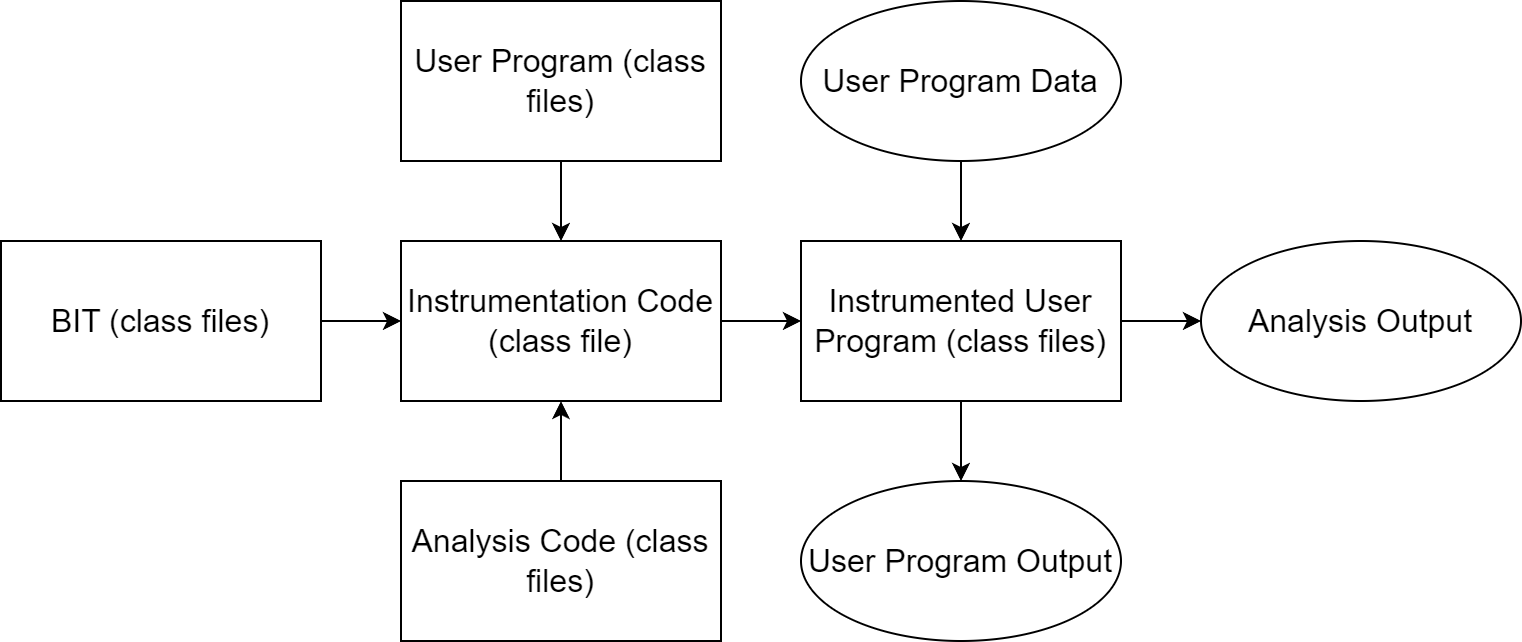
\includegraphics[width=.7\textwidth]{bit.png}
\caption{Архитектура фреймворка \texttt{BIT}.}
\label{fig:bitArch}
\end{figure}

На \autoref{fig:bitArch} проиллюстрирован процесс использования фреймворка \texttt{BIT}. Сначала пользователь пишет приложение, которое в последствии захочет инструментировать. Затем он пишет непосредственно код для инструментации и код для анализа бинарных файлов, используя классы и методы, предоставляемые фреймворком. Когда пользователь запустит код для инструментации, виртуальной машиной будут считаны бинарные файлы пользовательского приложения, после чего в нужные места пользовательского приложения будут вставлены вызовы кода для анализа. В результате получится инструментированное приложение, которое может впоследствии быть исполнено виртуальной машиной \texttt{Java}. Исполнение инструментированного приложения порождает как вывод оригинальной пользовательской программы, так и вывод анализа. Вставленные вызовы к функциям анализа ни коим образом не влияют на семантику приложения, и его вывод должен остаться неизменным.

Таким образом, \texttt{BIT} - это инструмент для создания специализированных инструментов для наблюдения и анализа поведения программ во время исполнения. \texttt{BIT} позволяет пользователям добавлять производить анализ в любом месте бинарного кода, а также получать динамическую информацию о программе во время исполнения. Подобные возможности делают \texttt{BIT} хорошим вариантом для имплементации профилировщиков и других схожих инструментов.

Ниже приведен пример того, как выглядит инструментация на фреймворке \texttt{BIT}. В \autoref{lst:Instrumentation} и \autoref{lst:Analysis} показано, каким образом будет выглядеть код для подсчета условных переходов во время исполнения.

\begin{lstlisting}[language=Java, caption=Подсчет условных переходов на \texttt{BIT}. Код инструментации, label=lst:Instrumentation]
    // filenameIn = ...; filenameOut = ...;
    ClassInfo ci = new ClassInfo(filenameIn);
    for (Enumeration e=ci.getRoutines().elements();e.hasMoreElements(); ){
        Routine routine = (Routine) e.nextElement();
        Vector instructions = routine.getInstructions();
        for (Enumeration b = routine.getBasicBlocks().elements(); b.hasMoreElements(); ) {
            BasicBlock bb = (BasicBlock) b.nextElement();
            Instruction instr = (Instruction)instructions.elementAt(bb.getEndAddress());
            short instr_type = InstructionTable.InstructionTypeTable[instr.getOpcode()];
            if (instr_type == InstructionTable.CONDITIONAL_INSTRUCTION) {
                instr.addBefore("BranchPrediction", "Offset", new Integer(instr.getOrigOffset()));
                instr.addBefore("BranchPrediction", "Branch", new String("BranchOutcome"));
            }
        }
        String method = new String(routine.getMethod());
        routine.addBefore("BranchPrediction", "EnterMethod", method);
        routine.addAfter("BranchPrediction", "LeaveMethod", method);
    }
    ci.write(filenameOut);
\end{lstlisting}

Заметим, что методы \texttt{addBefore} и \texttt{addAfter} добавляют вызовы к функциям, объявлены пользователем в коде анализа \autoref{lst:Analysis}.

\begin{lstlisting}[language=Java, caption=Подсчет условных переходов на \texttt{BIT}. Код анализа, label=lst:Analysis]
    public BranchPrediction {
        static Hashtable branch = null;
        static int pc = 0;
        public static void EnterMethod(String s) {
            branch = new Hashtable();
        }
        public static void LeaveMethod(String s) {
            System.out.println("stat for method: " + s);
            for (Enumeration e = branch.keys(); e.hasMoreElements(); ) {
                // Log results
            }
        }
        public static void Offset(int offset) {
            pc = offset;
        }
        public static void Branch(int brOutcome) {
            Branch b = (Branch) branch.get(pc);
            if (b == null)
                b = new Branch();
            if (brOutcome == 0)
                b.taken++;
            else
                b.not_taken++;
        }
    }
\end{lstlisting}

\subsection{BCA}

Фреймворк \texttt{BCA} помогает упростить составление связей между объектами путем смещения многих важных решений (например таких как имена методов или подтипирование) с времени разработки на время интеграции компонент, тем самым позволяя программистам адаптировать и применять даже сторонние библиотеки. 

\begin{figure}[h]
\centering
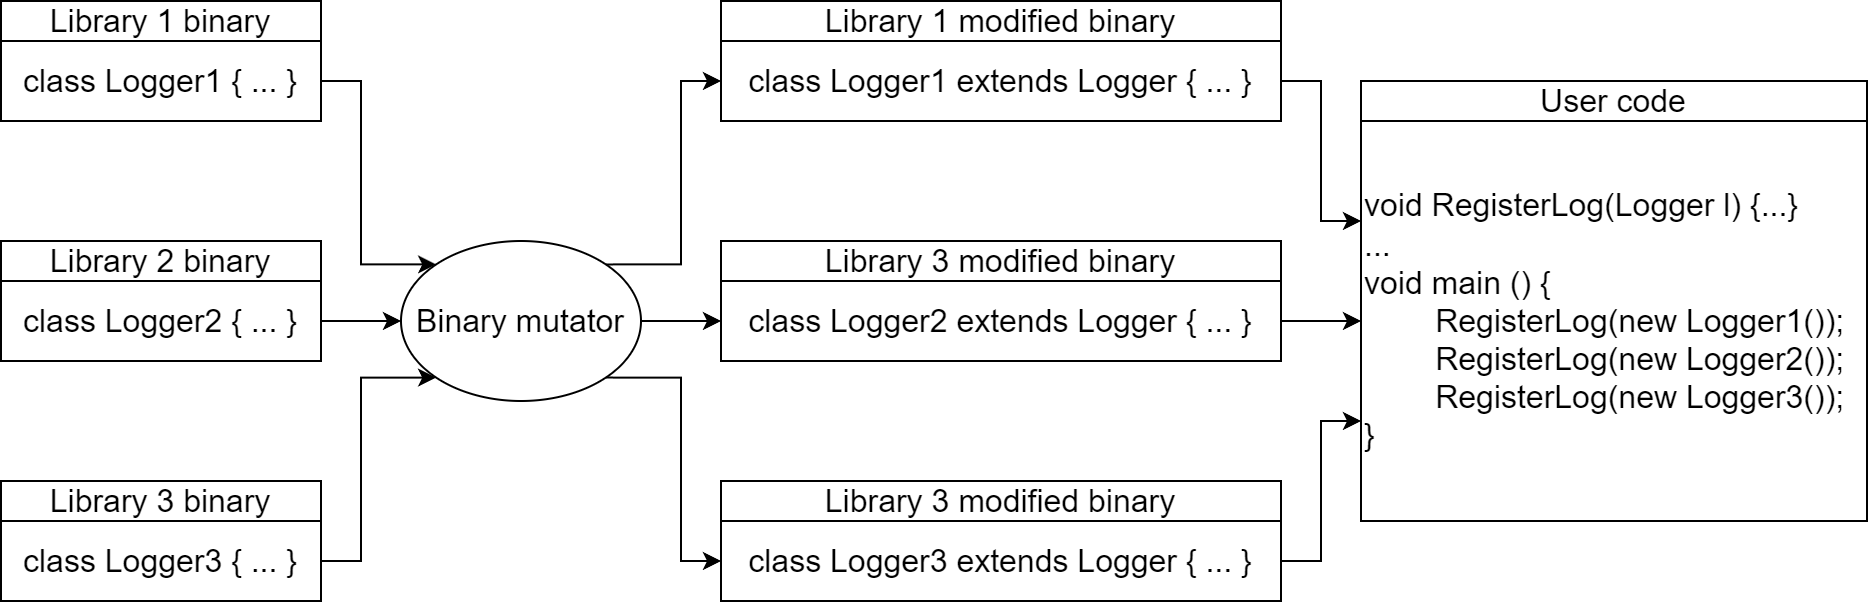
\includegraphics[width=.8\textwidth]{interoperability_example.png}
\caption{Пример использования фреймворка \texttt{BCA} для достижения интероперабельности сторонних компонент.}
\label{fig:interopExample}
\end{figure}

\texttt{BCA} изменяет компоненты во время их загрузки в виртуальную машину. Адаптация компонент происходит уже после того, как они были получены программистом, и их внутренняя структура модифицируется напрямую по месту использования. Вместо того, чтобы писать классы-обертки, происходит непосредственная модификация оригинального класса. Путем изменений бинарных файлов \texttt{BCA} удается достигнуть гибкости изменения исходного кода без сопуствующих этому недостатков:

\begin{itemize}
    \item Нет необходимости доступа к исходным файлам, что позволяет использовать фреймфорк даже на сторонних библиотеках
    \item Модификация может быть отложена до времени загрузки, что позволяет применять их по месту использования.
    \item В сравнении с модификацией исходного файла приводит к меньшему приросту времени загрузки.
    \item Модификация бинарного файла очень гибкая, и позволяет легко производить многие операции, такие как добавление нового метода, переименовывание, изменение подтипирования и иерархии классов.
\end{itemize}

Общая структура фреймворка \texttt{BCA} и его интеграция в виртуальную машину \texttt{Java} проиллюстрированы на \autoref{fig:bcaArch}.

\begin{figure}[h]
\centering
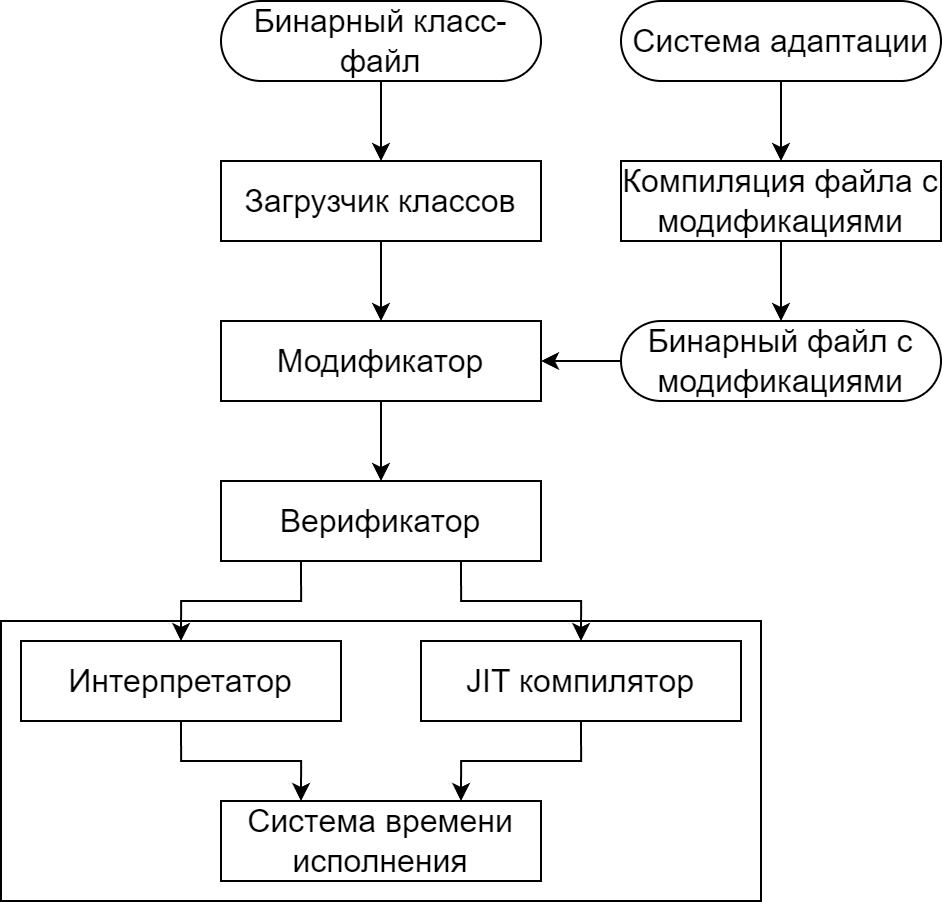
\includegraphics[width=.55\textwidth]{bca.png}
\caption{Архитектура фреймворка \texttt{BCA}.}
\label{fig:bcaArch}
\end{figure}

Когда загрузчик класс-файлов считывает бинарный файл, он сторит внутреннее представление для этого файла. Во время обычного исполнения виртуальной машины \texttt{Java} это внутреннее представление сразу передается верификатору. \texttt{BCA} встраивает между этими двумя этапами, перенаправляя промежуточное представление модификатору, применяющему все необходимые трансформации к класс файлу. Все трансформации описаны в файле с модификациями (\texttt{Delta~File}), который считывается модификатором при запуске виртуальной машины. 

После модификации изменное представление класса передается верификатору, который проверяет код на соответствие спецификации \texttt{JVM} с целью выявления недопустимых операций. После успешной верификации промежуточное представление передается в часть \texttt{JVM}, отвечающую за время исполнения. \texttt{BCA} не требует никаких изменений ни в веривикатор \texttt{JVM}, ни в часть, отвечающую за время исполнения, что делает его применение более портабельным.

Чтобы гарантировать консистентность изменений, системе адаптации нужно иметь доступ ко всем файлам, которые могут быть потенциально затронуты изменениями. В случае, если весь проект хранится локально, то может быть произведена статическая адаптация компонент, в ходе которой \texttt{BCA} может просто считать все файлы и заранее применить к ним необходимые изменения, получив при этом цельное измененное приложение. Статическая адаптация имеет недостаток в том, что ей требуется дополнительное место на хранение измененного приложения, что приводит к большему потреблению дискового пространства. Однако статическая адаптация полностью убирает какие либо дополнительные затраты при загрузке классов, т.к. вссе трансформации уже были применены. Более того, такая адаптация позволяет публиковать код без необходимости изменений среды на стороне конечного пользователя.

Альтернативой статической адаптации является динамическая адаптация. Динамическая адаптация работает по схеме, приведенной на \autoref{fig:bcaArch}, тоесть производит все манипуляции во время исполнения. Такой подход приводит к дополнительным расходам во время загрузки, что приводит к увеличению общего времени исполнения. Также динамическая адаптация требует того, чтобы файлы с модификациями распространялись вместе с приложением, и конечный пользователь использовал систему с предустановленным \texttt{BCA}. С другой стороны, динамическая адаптация не требует дополнительного места на хранение модифицированной копии приложения. Более того, в данном подходе не требуется апиорное знание всвех методов, которые будут загружены в приложении, что позволяет поддержать более сложные сценарии с динамической загрузкой классов (например стандартный метод \texttt{Class.forName} позволяет искать класс по имени, производя динамическую загрузку, если до этого ее не было произведено. Поскольку аргумент данной функции - строка, то не всегда есть возможность статически вычислить, чему будет равно ее значение, и статической адаптации будет недостаточно \cite{bca}).

\subsection{Kava}

Примером фреймворка, расширящего стандартные средства рефлексии языка является \texttt{Kava} \cite{kava1} \cite{kava2}. Большинство фреймворков для манипуляции байткодом предоставляют объектно-ориентированное представление для элементов бинарного класс-файла таких как методы, типы, инструкции и других. После чего пользователю предлагается написать отдельную программу, описывающую, как переписать класс файл. Главным недостатком данного подхода является то, что для того чтобы им возпользоваться, пользователь должен обладать знаниями о байткода и формате бинарного файла платформы. Альтернативныс является подход, оперирующий на языковом уровне, что несколько обезопасит и облегчит использование программистом бинарного кода. Поэтому \texttt{Kava} предлагает модель на основе поведенческой рефлексии, позволяющая изменять поведение приложения без необходимости изменения имплементации всей программы.

Для представления языковых сущностей \texttt{Kava} использует метаобъекты (\texttt{Meta~Object~Protocol}). При их помощи поведение сущностей во время исполнения, например доступ к полю, вызов метода и другие, могут быть переопределены. Метаобъекты конструируются при помощи овеществления (reification) рантайм модели объектов. Например, метод овеществляется как объект класса \texttt{Method}.

\begin{figure}[h]
\centering
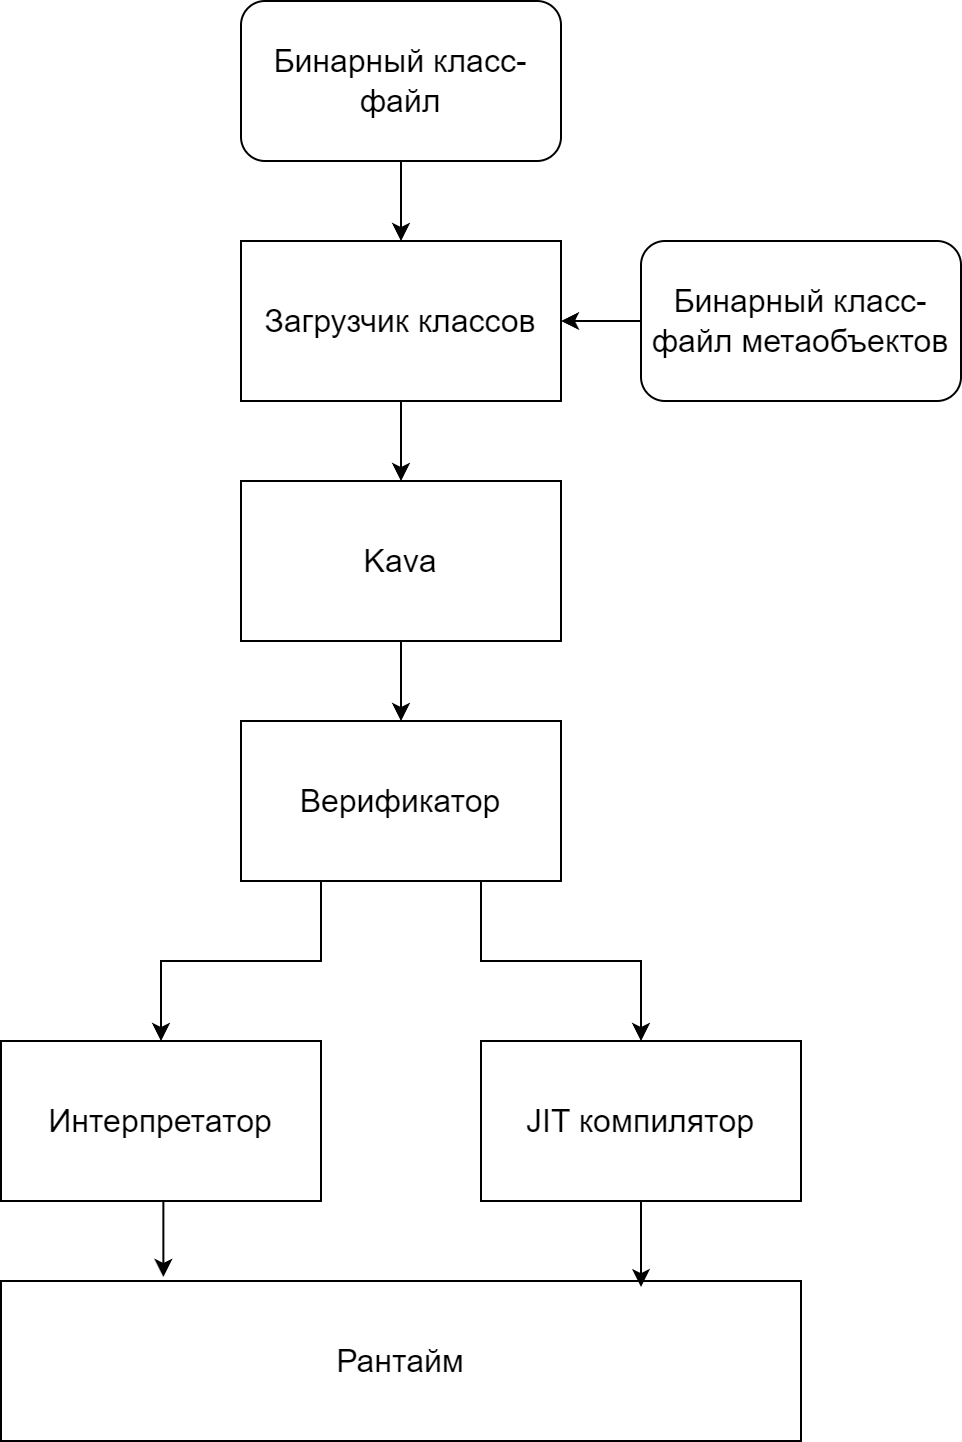
\includegraphics[width=.45\textwidth]{kava.png}
\caption{Архитектура фреймворка \texttt{Kava}.}
\label{fig:kavaArch}
\end{figure}

Как видно из \autoref{fig:kavaArch}, \texttt{Kava} реализована при помощи инструментирования класс файла кодом, передающим контроль метаобъекту, ассоциированному с объектом. Для манипуляции самим байткодом \texttt{Kava} использует сторонний низкоуровневый фреймворк \texttt{BCEL}. При помощи него \texttt{Kava} инструментирует класс-файл во время его загрузки, что позволяет пользователю перехватывать и переопределять такие события как доступ к полю класса, вызов метода, вызов конструктора или выброс программой исключения.

Ниже в \autoref{lst:kava1} представлен простой пример работы с \texttt{Kava}. В нем пользователь хочет перехватить исполнение метода, пожтому он переопределяет процесс исполнения функций платформой, исполняющей \texttt{Java}. Перед исполнением функции будут выведены ее имя и дополнительная информация.

\begin{lstlisting}[language=Java, caption=Объявление метаобъекта в \texttt{Kava}, label=lst:kava1]
    public class TracingMetaObject implements MetaObject {
        public ExecutionContext beforeExecuteMethod(ExecutionContext context) {
            System.out.println("tracing " + context.getMethodName());
        }
    };
\end{lstlisting}

Для достижения желаемого результата, метаобъект должен быть привязан к классу, вызов методов которого необходимо отслеживать. Код, приведенный в \autoref{lst:kava2}, показывает как добиться отслеживания вызовов всех методов класса \texttt{Test}.

\begin{lstlisting}[language=Java, caption=Привязка класса к метаобъекту в \texttt{Kava}, label=lst:kava2]
    bind {
        class Test metaclass-is TracingMetaObject {
            any-method(any-parameters) {
                execute;
            }
        }
    }
\end{lstlisting}

Для сравнения, имплементация эквивалентной логики при помощи классического фреймворка для работы с класс-файлами приведен ниже в \autoref{lst:kava3}

\begin{lstlisting}[language=Java, caption=Реализация аналогичной функциональности при помощи классического фреймворка для работы с класс-файлом, label=lst:kava3]
    public class TraceMethod implements Constants {
        private static Method traceMethod(Method m) {
            // create the byte code to insert
            // find insertion point
            // insert byte code at beginning of method
            // recalculate stack size
            // return modified method
        }
        public static void main(String[] argv) {
            // parse the class
            // get constant pool
            // generate necessary constants
            // foreach method:
            // call traceMethod
            // write out modified class
        }
    }
\end{lstlisting}

У данного подхода есть несколько недостатков в сравнении с реализацией через расширенный механизм рефлексии. Во первых, программист должен самостоятельно генерировать инструкции, которые необходимо вставить в бинарное представление методов, а также самостоятельно обходить класс-файл чтобы найти нужную точку вставки нового кода. Вдобавок, вставленный код может быть верифицирован только при повторной загрузке класс-файла. При помощи расширения механизма рефлексии бинарной манипуляцией, этих недостатков удается избежать.

\subsection{AspectJ}

\texttt{AspectJ} является расширением для языка \texttt{Java}, привнося в него поддержку элементов аспекто-ориентированного программирования. Данное расширение вносит в язык следующие понятия и сущности \cite{aspectj}:

\begin{itemize}
    \item Точки соединения (\texttt{Join~Points}) - однозначно определенные точки в исполнении программы.
    \item Срез (\texttt{Pointcut}) - ссылка на набор точек соединения и значения, определенные в них.
    \item Совет (\texttt{Advice}) - функционал, который определяет поведение в точке соединения.
    \item Аспект (\texttt{Aspect}) - модуль, реализующий сквозную функциональность. Аспект отвечает за применение некоего совета в точках соединения, которые определяются некоторым срезом
\end{itemize}

Далее будет приведен краткий обзор каждого из этих понятий.

Модель точки соединения является критичным элементом в любой аспекто-ориенттированной системе. Данная модель предоставляет общую "систему координат", позволяющую координировать исполнение аспектов. \texttt{AspectJ} имплементирует модель, в которой точки соединения - это некоторые одозначно определенные точки в исполнении программы. В грубом приближении точки соединения в \texttt{AspectJ} можно представлять как узлы в графе потока управления. Получается, что поток управления проходит через каждую точку соединения дважды: первый раз на пути в поддерево, и второй раз - на обратном пути. \texttt{AspectJ} выделяет следующие виды точек соединения:

\begin{itemize}
    \item Вызов метода или конструктора - данная точка соединения находится на стороне вызывающего объекта, сразу до вызова метода или конструктора.
    \item Принятие вызова метода или конструктора - данная точка соединения находится на стороне вызываемого объекта, и находится строго до вызова метода / конструктора.
    \item Исполнение метода или конструктора - данная точка соединения находится в вызываемом методе или конструкторе
    \item Чтение или запись поля
    \item Вызов обработчика исключений
    \item Инициализация класса
    \item Инициализация объекта
\end{itemize}

Срез, как уже было сказано, это набор точек соединения с, возможно, некоторыми значениями из контекста исполнения в этих точках соединения. \texttt{AspectJ} определяет несколько примитивных срезов, которые пользователь может комбинировать, чтобы создавать свои виды срезов. Например срез $receptions(void Point.setX(int))$ объединяет все точки соединения вида "Принятие вызова метода или конструктора", в которых сигнатура принимаемого метода равна $void Point.setX(int)$. Срезы могут комбинироваться с помощью логических операторов, как показано ниже:

\begin{lstlisting}[language=Java, caption={Срез, следящий за координатой точки \texttt{x} или \texttt{y}.}]
    receptions(void Point.setX(int)) || receptions(void Point.setY(int))
\end{lstlisting}

Пользователь также может определять собственные срезы:

\begin{lstlisting}[language=Java, caption={Пользовательский срез, следящий за координатой точки \texttt{x} или \texttt{y}.}]
    pointcut moves():
        receptions(void FigureElement.incrXY(int, int)) ||
        receptions(void Line.setP1(Point)) ||
        receptions(void Line.setP2(Point)) ||
        receptions(void Point.setX(int)) ||
        receptions(void Point.setY(int));
\end{lstlisting}

Совет - это функциональный механизм, использующийся для декларации логики, вызываемой в каждой из точек соединения в срезе. \texttt{AspectJ} определяет три вида советов - \texttt{before}, \texttt{after} и \texttt{around}. Совет определяется путем соотнесения куска кода с срезом и промежутком времени, относительно которого должен будет быть применен код в каждой из точек соединения. Например совет:

\begin{lstlisting}[language=Java, caption={Совет, отмечающий изменения точки \texttt{x} или \texttt{y}.}]
    after(): moves() {
        flag = true;
    }
\end{lstlisting}

определяет совет в срезе \texttt{moves()}. Этот совет выставляет флаг каждый раз когда исполнение выйдет из среза \texttt{moves()}.

Аспекты - это модули, определяющие сквозную логику. Декларация аспекта ведет себя как декларация класса. Внутри него могут быть определены срезу, советы и другие декларации, допустимые внутри класса. Ниже приведен пример декларации аспекта, следящего за тем, была ли фигура передвинута.

\begin{lstlisting}[language=Java, caption={Аспект, отслеживающий изменения фигур.}]
aspect MoveTracking {
    static boolean flag = false;
    static boolean testAndClear() {
        boolean result = flag;
        flag = false;
        return result;
    }
    pointcut moves():
        receptions(void FigureElement.incrXY(int, int)) ||
        receptions(void Line.setP1(Point)) ||
        receptions(void Line.setP2(Point)) ||
        receptions(void Point.setX(int)) ||
        receptions(void Point.setY(int));
    after(): moves() {
        flag = true;
    }
}
\end{lstlisting}


Советы аспекта чем-то похожи на методы в том смысле что имеют доступ к всем членам аспекта. В данном случае совет \texttt{after()} может спокойно работать со статическим полем \texttt{flag}.

Как видно из примеров, применение \texttt{AspectJ} позволяет имплементировать сквозную логику в виде отдельных модулей, тем самым явно выражая ее в одном месте. Благодаря этому, различные инструменты имеют возможность понимать сквозную логику проекта и давать программисту релевантные подсказки.

\subsection{Javassist}

Подобно \texttt{AspectJ}, \texttt{Javassist} является расширением языка \texttt{Java}, с той лишь разницей, что \texttt{Javassist} ставит своей целью расширить возможности встроенного функционала рефлексии. Данный вреймворк, как и \texttt{BCA}, может быть применен как статически, так и динамически. \texttt{Javassist} был разработать с целью упростить и безопасить процесс инструментации финарного файла и убрать необходимость рядовому разработчику проникать в детали работы виртуальной машины. Поэтому для имплементации этого фреймворка был выбран уровень абстракции исходного кода. Этот выбор приводит к уменьшению гибкости интерфейса, но с другой стороны позволяет сделать его более удобным для разработчика. Также в \texttt{Javassist} существует набор методов, позволяющих работать с байткодом напрямую. Помимо предоставления абстракций на уровне исходного кода, \texttt{Javassist} автоматически обновляет места использования модифицированных сущностей. Например, если имя класса было изменено, то оно будет изменено и в тех местах, где это имя используется.

Для работы с исходным кодом \texttt{Javassist} не использует полноценный java компилятор, поскольку полноценная компиляция \texttt{Java} кода довольно медленный процесс, и как правило, для работы функций фреймворка требуется скомпилировать только тело метода, не создавая при этом классов и другие вспомогательные структуры, которые присутствуют в бинарном класс-файле. Для обеспечения быстродействия компиляции, \texttt{Javassist} использует собственный компилятор, транслирующий только тело метода и вставляет его байткод в уже сущестующий метод.

Для обеспечения безопасности трансформаций, \texttt{Javassist} позволяет производить только ограниченный набор изменений. Например, в классе невозможно удалить поле или метод, можно только изменить тело уже существующего метода, или нельзя изменять сигнатуру существующего метода.

Приведем пример пользования данного фреймворка для инструментации кода. Рассмотрим пример, в котором пользователь выводит значения аргументов функциии. Пусть есть метод, описанный в \autoref{lst:javassistExample}.

\begin{lstlisting}[language=Java, caption=Исходный класс, label=lst:javassistExample]
public class Point {
    int x, y;
    void move(int dx, int dy) {
        x += dx; y += dy;
    }
}
\end{lstlisting}

Для вставки логгирующего кода, пользователь должен написать последовательность инструкций, описанную на \autoref{lst:javassistCode}.

\begin{lstlisting}[language=Java, caption={Код, добавляющий логгирование}, label=lst:javassistCode]
    // ...
    ClassPool pool = ClassPool.getDefault();
    CtClass cc = pool.get("Point");
    CtMethod m = cc.getDeclaredMethod("move");
    m.insertBefore("{ System.out.println($1); System.out.println($2); }");
    cc.writeFile();
    // ...
\end{lstlisting}

\subsection{ASM}

Аналогично \texttt{BCA}, ферймворк \texttt{ASM} \cite{asm} поддерживает как статический режим трансформации, так и динамический, являющийся для \texttt{ASM} основным режимом работы. Поэтому как имплементация фреймворка, так и его пользовательский интерфейс заточены под то, чтобы уменьшить дополнительные расходы на работу с класс-файлами во время загрузки.

\texttt{ASM} поддерживает два варианта пользовательского интерфейса: событийный и объектно-ориентированный. Рассмотрим каждый из них по отдельности.

Событийный пользовательский интерфейс является изначальным интерфейсом \texttt{ASM} и призван решить главную проблему объекто-ориентированного представления: создание большого числа объектов для репрезентации элементов класса при загрузке, что приводит к падению производительности и увеличению расходов памяти виртуалььной машины. Данный интерфейс реализован при помощи шаблона посетитель (\texttt{Visitor~Design~Pattern}). Применение данного шаблона позволяет изменять как бинарный код методов, так и структуру класса без необходимости создания объекта на каждую из сущностей, что позволяет \texttt{ASM} значительно уменьшить накладные расходы при загрузке классов.

Объектно-ориентированный интерфейс представляет класс в виде дерева объектов, в котором каждый объект осуществляет некую сущность принадлежащую классу, такую как сам класс, его поле, метод, и другие. Каждый объект содержит ссылки на объекты, осуществляющие принадлежащие ему сущности. Помимо этого, объектно-ориентированный интерфейс предоставляет функционал для преобразования древовидного представления в событийное и обратно. Другими словами, объектно-ориентированный интерфейс реализован поверх событийного интерфейса.

Каждый из этих интерфейсов имеет как свои преимущества, так и свои недостатка. Например, как было сказано выше, событийный интерфейс работает быстрее и требует меньше памяти, чем объектно-ориентированный. Однако такой интерфейс пригоден только для написания достаточно простых преобразований, поскольку в любой момент доступен только один из элементов класса, соответствующий текущему посещаемому элементу. Объектно-ориентированный интерфейс решает эту проблему, предоставляя пользователю доступ сразу ко всей модели класса, но ценой дополнительных расходов на построение дерева объектов.

Сравним эти два интерфейса на следующем примере. Пусть пользователю нужно создать код для метода в \autoref{lst:asmfoo}

\begin{lstlisting}[language=Java, caption=Необходимый метод., label=lst:asmfoo]
public class MyClass {
    int fld = 1;
    public int getFld() {
        return this.fld;
    }
}
\end{lstlisting}

Используя событийный интерфейс, создание инструкций данного метода достигается следующей последовательностью вызовов \autoref{lst:asmVisitor}.

\begin{lstlisting}[language=Java, caption=Пример использования событийного интерфейса., label=lst:asmVisitor]
    mv.visitCode();
    mv.visitVarInsn(ALOAD, 0);
    mv.visitFieldInsn(GETFIELD, "pkg/MyClass", "fld", "I");
    mv.visitInsn(IRETURN);
    mv.visitMaxs(1, 1);
    mv.visitEnd();
\end{lstlisting}

Ту же самую логику можно выразить при помощи объектно-ориентированного интерфейса \autoref{lst:asmOOP}.

\begin{lstlisting}[language=Java, caption=Пример использования объектно-ориентированного интерфейса., label=lst:asmOOP]
    MethodNode mn = new MethodNode(/* ... */);
    InsnList il = mn.instructions;
    il.add(new VarInsnNode(ILOAD, 1));
    LabelNode label = new LabelNode();
    il.add(new JumpInsnNode(IFLT, label));
    il.add(new VarInsnNode(ALOAD, 0));
    il.add(new VarInsnNode(ILOAD, 1));
    // ...
\end{lstlisting}

Интерфейс для работы с инструкциями автоматически осуществляет поддержку таких служебных сущностей как constant pool. Проведение анализа потока управления осуществляется при помощи отдельной функциональности \texttt{ASM}, позволяющей строить графовое представление функций. Анализ же потока данных осуществляется при абстрактной интерпретации, позволяющей смоделировать все возможные пути исполнения инструкций в методе для получения всех возможных значений ее аргументов.

\subsection{Анализ существующих решений}

Все рассмотренные в данном разделе решения можно сравнивать по множеству признаков, таких как уровень абстракции сущностей, назначение фреймворка, требуется ли глубокое знание бинарного кода для работы с ним, и дргуим. В ходе данной работы такое сравнение было проведено, в результате чего была получена следующая таблица:

\begin{figure}[h]
\centering
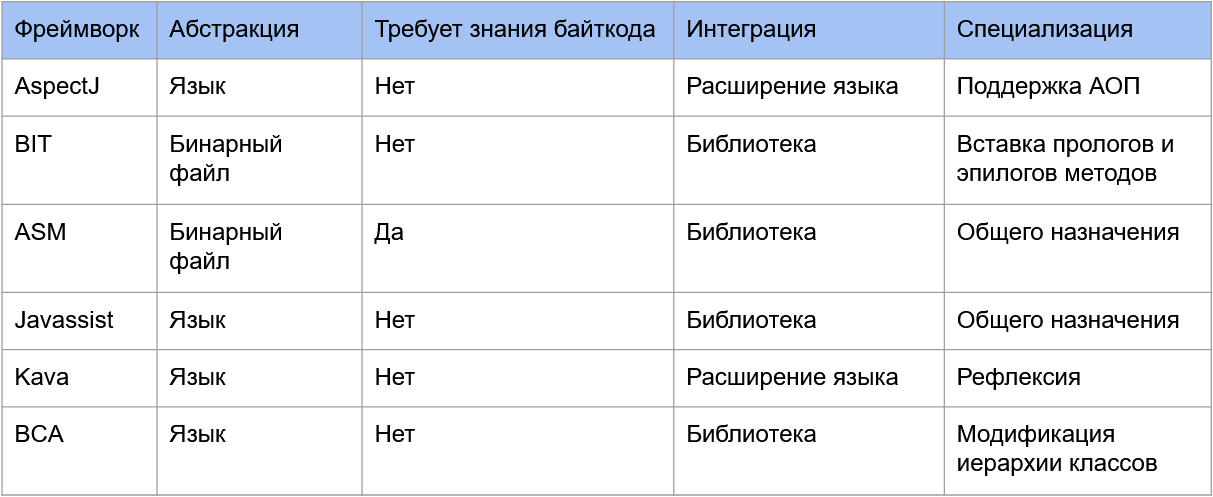
\includegraphics[width=\textwidth]{framework_comparison.png}
\caption{Сравнение рассмотренных фреймворков.}
\label{fig:kavaArch}
\end{figure}

Изучив ее и требования, выдвинутые при построении задачи, был сделан вывод, что ни одно из существующих решений не выполняет в полной мере поставленные перед данной работой задачи, из-за чего требуется более детальное рассмотрение каждого из фреймворков по отдельности и выделение из его архитектуры необходимых нам аспектов.

\newpage
